102. \begin{figure}[ht!]
\center{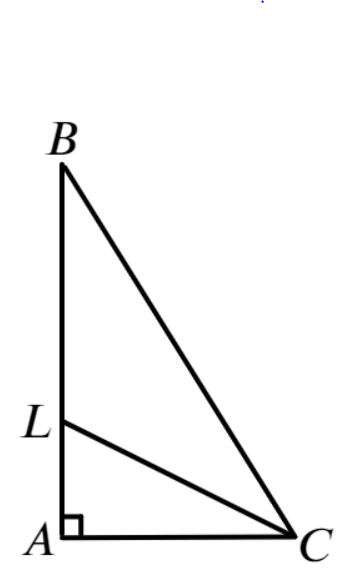
\includegraphics[scale=0.35]{g9-102.png}}
\end{figure}\\
По теореме Пифагора имеем $AB=\sqrt{625-49}=24$см. По свойству основания биссектрисы получаем соотношение $\cfrac{AL}{LB}=\cfrac{AC}{BC}=\cfrac{7}{25},$ значит $AL=\cfrac{7}{32}\cdot24=\cfrac{21}{4}$см. Тогда  по теореме Пифагора $CL=\sqrt{\cfrac{441}{16}+49}=\cfrac{35}{4}$см.\newpage\noindent
